% =====================================================================
%  SLIDE THUYẾT TRÌNH (16:9). Số liệu giống bản báo cáo cập nhật (_v2), thêm điện thoại phổ thông TCL T506T.
%  Số đo của TCL nằm trong ../so_lieu_tcl.tex (sinh bởi ../make_tcl.py từ results/phone/tcl).
%  Biên dịch (2 lần): pdflatex -jobname="24119068_Huỳnh Lê Thành Nhân_Slide" vieedge_slides.tex
% =====================================================================
\documentclass[aspectratio=169,11pt]{beamer}
\usepackage[T5]{fontenc}
\usepackage[utf8]{inputenc}
\usepackage[vietnamese]{babel}
\usepackage[scaled=.95]{helvet}
\usepackage{graphicx,booktabs,array,amsmath,amssymb,tikz}
% Thông tin chung cho bài báo và poster: sửa một chỗ ở đây.
\newcommand{\tenviet}{VieEdge-Voice: Trợ lý hỏi đáp bằng giọng nói tiếng Việt chạy hoàn toàn offline trên thiết bị biên}
\newcommand{\TENVIET}{VIEEDGE-VOICE: TRỢ LÝ HỎI ĐÁP BẰNG GIỌNG NÓI TIẾNG VIỆT CHẠY HOÀN TOÀN OFFLINE TRÊN THIẾT BỊ BIÊN}
\newcommand{\tenanh}{VieEdge-Voice: a fully offline Vietnamese voice question-answering assistant on edge devices}
\newcommand{\svmot}{Huỳnh Lê Thành Nhân}
\newcommand{\mssvmot}{24119068}
\newcommand{\svhai}{Nguyễn Đoàn Hoàng Ngân}
\newcommand{\mssvhai}{24119064}
\newcommand{\emailmot}{24119068@student.hcmute.edu.vn}
\newcommand{\truong}{Trường Đại học Công nghệ Kỹ thuật Thành phố Hồ Chí Minh}
\newcommand{\khoa}{Khoa Đào tạo tiên tiến}
\definecolor{xanhute}{HTML}{0272BC}
\definecolor{doute}{HTML}{D3202A}
\definecolor{dam}{HTML}{0B3C78}

% Sinh tự động bởi make_tcl.py từ results/phone/tcl; không sửa tay.
\newcommand{\tclChip}{Helio P22 (MT6762), 8 lõi Cortex-A53}
\newcommand{\tclRam}{4 GB}
\newcommand{\tclParity}{2.474/2.474}
\newcommand{\tclParityMs}{30\,ms}
\newcommand{\tclSafeOk}{20/24}
\newcommand{\tclSafeOkB}{20/24}
\newcommand{\tclSafeMed}{1,43}
\newcommand{\tclSafeHi}{1,67}
\newcommand{\tclSafeMax}{1,75}
\newcommand{\tclSttMed}{1,33}
\newcommand{\tclFourMed}{1,53}
\newcommand{\tclFourOk}{20/24}
\newcommand{\tclGreedyMed}{1,33}
\newcommand{\tclGrOk}{19/24}
\newcommand{\tclSttNote}{3 luồng 1,43\,s, 4 luồng 1,53\,s, 4 luồng không thiên vị từ khoá 1,33\,s (19/24 đúng thẻ).}
\newcommand{\tclLoadA}{68}
\newcommand{\tclLoadB}{100}
\newcommand{\tclTokA}{3,1}
\newcommand{\tclTokB}{1,8}
\newcommand{\tclAnsA}{12,64}
\newcommand{\tclAnsB}{22,53}
\newcommand{\tclFirstA}{1,99}
\newcommand{\tclFirstB}{2,03}
\newcommand{\tclPssA}{1,3}
\newcommand{\tclPssB}{2,0}
\newcommand{\tclTempA}{35,5}
\newcommand{\tclTempB}{36,5}
\newcommand{\tclNqa}{8}
\newcommand{\tclNqb}{8}
\newcommand{\tclAnsRag}{23,18}
\newcommand{\tclTtftRag}{11,6}
\newcommand{\tclPromptRag}{106}
\newcommand{\tclTtftA}{2,9}
\newcommand{\tclAnsEight}{72,51}
\newcommand{\tclTokEight}{1,2}
\newcommand{\tclBest}{4 luồng, không thiên vị}
\newcommand{\tclTakeaway}{Máy phổ thông vẫn trả lời được offline, nhưng chậm: mô hình 0,8 tỉ cho câu trả lời thật sau 12,64\,s (trung vị, 8 câu, tắt tra cứu), bật tra cứu thì 23,18\,s vì CPU chỉ nạp khoảng 9 token prompt mỗi giây; mô hình 2 tỉ sau 22,53\,s. Câu khẩn cấp không qua LLM nên vẫn có tiếng sau 1,43\,s.}

% Sinh tự động bởi make_hai_may.py; không sửa tay.
\newcommand{\hmAsrF}{65}
\newcommand{\hmAsrT}{889}
\newcommand{\hmAsrRtfF}{0,022}
\newcommand{\hmAsrRtfT}{0,305}
\newcommand{\hmTtsF}{270}
\newcommand{\hmTtsT}{2274}
\newcommand{\hmTtsRtfF}{0,087}
\newcommand{\hmTtsRtfT}{0,722}
\newcommand{\hmSafeMsF}{3,0}
\newcommand{\hmSafeMsT}{27,1}
\newcommand{\hmPpF}{454}
\newcommand{\hmPpT}{10,8}
\newcommand{\hmTgF}{79,5}
\newcommand{\hmTgT}{4,6}
\newcommand{\hmPpBF}{196}
\newcommand{\hmPpBT}{4,3}
\newcommand{\hmTgBF}{28,2}
\newcommand{\hmTgBT}{2,2}
\newcommand{\hmLoadF}{5}
\newcommand{\hmLoadT}{68}
\newcommand{\hmSafeF}{0,48}
\newcommand{\hmSafeT}{1,43}
\newcommand{\hmSafeOkF}{20/24}
\newcommand{\hmSafeOkT}{20/24}
\newcommand{\hmAnsF}{1,4}
\newcommand{\hmFirstF}{0,59}
\newcommand{\hmTtftF}{0,2}
\newcommand{\hmPssF}{1,9}
\newcommand{\hmAnsT}{12,6}
\newcommand{\hmFirstT}{1,99}
\newcommand{\hmTtftT}{2,9}
\newcommand{\hmPssT}{1,3}
\newcommand{\hmSpeedup}{9}

\graphicspath{{../figures/}}
\usefonttheme{professionalfonts}
\setbeamertemplate{navigation symbols}{}
\setbeamercolor{frametitle}{fg=dam}
\setbeamercolor{title}{fg=dam}
\setbeamercolor{structure}{fg=xanhute}
\setbeamercolor{normal text}{fg=black!88}
\setbeamerfont{frametitle}{size=\Large,series=\bfseries}
\setbeamertemplate{itemize item}{\color{xanhute}$\blacksquare$}
\setbeamertemplate{itemize subitem}{\color{doute}\textbullet}
\setbeamertemplate{frametitle}{\vspace{4pt}\insertframetitle\par\vspace{-3pt}{\color{doute}\rule{28mm}{1mm}}}
\setbeamertemplate{footline}{\hfill{\scriptsize\color{black!50}\insertframenumber/\inserttotalframenumber}\hspace{8pt}\vspace{5pt}}
\newcommand{\so}[2]{\begin{minipage}[t]{.23\linewidth}\centering{\Huge\bfseries\color{xanhute}#1}\par\vspace{3pt}{\small #2}\end{minipage}}
\newcolumntype{R}[1]{>{\raggedleft\arraybackslash}p{#1}}

\begin{document}

% ------------------------------------------------------------------ 1
\begin{frame}[plain]
\vspace{-4pt}

\includegraphics[height=13mm]{logo_truong.png}\hfill
\includegraphics[height=13mm]{logo_khoa_vuong.png}
\vspace{10pt}
\begin{center}
{\Large\bfseries\color{dam}\TENVIET\par}
\vspace{8pt}
{\normalsize\color{black!70}\tenanh\par}
\vspace{16pt}
{\large\textbf{\svmot} (MSSV \mssvmot)\quad \textbf{\svhai} (MSSV \mssvhai)\par}
\vspace{6pt}
{\small\khoa, \truong\par}
\end{center}
\end{frame}

% ------------------------------------------------------------------ 2
\begin{frame}{Đặt vấn đề}
\begin{columns}[T]
\begin{column}{.56\textwidth}
\begin{itemize}
\item Trợ lý giọng nói phổ biến chạy trên đám mây: mất mạng là ngừng, giọng nói phải rời máy.
\item Mạng hay mất đúng lúc cần nhất: bão lũ, sạt lở cắt sóng và điện, người dân cần hỏi cách sơ cứu, thoát hiểm ngay.
\item Người nói chỉ chờ vài trăm mili giây giữa hai lượt lời, nên trợ lý bị đánh giá bằng thời gian chờ.
\item Trên thiết bị biên, mô hình phổ thông sai nhiều với tiếng Việt (Whisper-tiny sai 53\% số từ trên VIVOS).
\end{itemize}
\end{column}
\begin{column}{.40\textwidth}
\begin{block}{Câu hỏi của đề tài}
Một thiết bị biên có thể nghe, hiểu và trả lời bằng tiếng Việt, hoàn toàn không Internet, đủ nhanh để hội thoại và đủ an toàn khi khẩn cấp hay không?
\end{block}
\end{column}
\end{columns}
\end{frame}

% ------------------------------------------------------------------ 3
\begin{frame}{Sản phẩm và đóng góp}
\begin{itemize}
\item Đường ống ngoại tuyến đầu cuối: Silero VAD, Zipformer, tra cứu Wikipedia, LLM Qwen3.5 tinh chỉnh LoRA, TTS Piper.
\item Ba thiết bị, cùng quy ước đo: Raspberry Pi 5 với Yocto PREEMPT\_RT; Galaxy Z Fold7 dùng NPU Hexagon; điện thoại phổ thông TCL T506T chỉ có CPU.
\item 85 thẻ sơ cứu, thiên tai và an toàn viết lại từ 82 nguồn, kể cả tình huống ở nước ngoài; câu khẩn cấp không để LLM tự viết.
\item Ứng dụng Android: chạm để nói, lịch sử trò chuyện, \textbf{vị trí GPS và bản đồ ngoại tuyến} cho vùng không có sóng.
\item Kết quả âm được công bố: Hailo-8L, giải mã suy đoán, lời nhắc ``nói thẳng'' và Gemma trên điện thoại đều đã thử và không dùng.
\end{itemize}
\end{frame}

% ------------------------------------------------------------------ 4
\begin{frame}{Lưu đồ một lượt hỏi}
\centering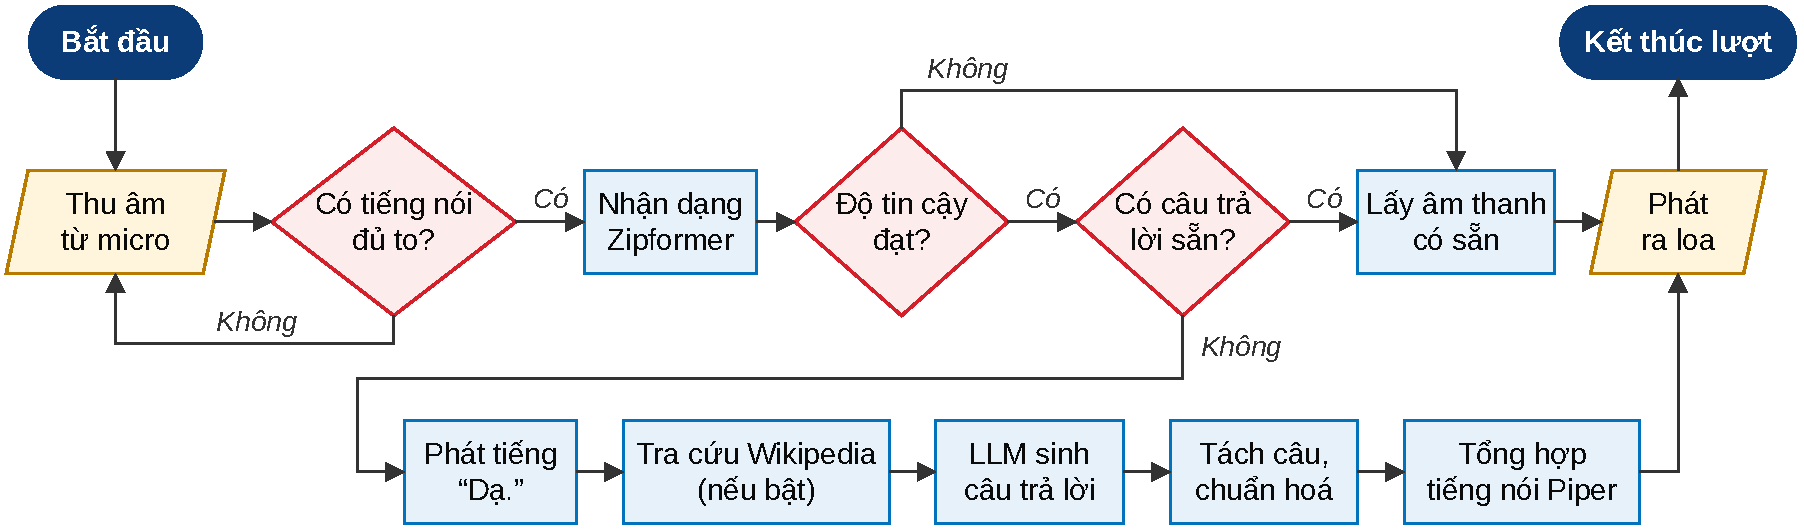
\includegraphics[width=.96\textwidth]{luu_do.pdf}\par\vspace{4pt}
{\small Câu khẩn cấp đi nhánh thẻ an toàn trước tiên; câu có sẵn đi nhánh nhanh; còn lại qua tra cứu, LLM và TTS theo cơ chế luồng.}
\end{frame}

% ------------------------------------------------------------------ 5
\begin{frame}{Ba nền tảng}
\centering\footnotesize
\begin{tabular}{@{}l>{\centering\arraybackslash}p{34mm}>{\centering\arraybackslash}p{38mm}>{\centering\arraybackslash}p{38mm}@{}}\toprule
 & Raspberry Pi 5 & Galaxy Z Fold7 & TCL T506T\\\midrule
Chip & Cortex-A76 $\times$4 & Snapdragon 8 Elite & Helio P22, 8 lõi Cortex-A53\\
Tăng tốc & Hailo-8L (chưa dùng được) & NPU Hexagon v79, GPU Adreno & không (chỉ CPU)\\
RAM & 8 GB & 12 GB & \tclRam\\
Hệ điều hành & Yocto PREEMPT\_RT & Android 16 & Android 13\\
Bản llama.cpp & ARMv8.2 dotprod & ARMv8.7 + NPU, GPU & ARMv8.0 (bản riêng)\\
LLM mặc định & 0,8 tỉ & 2 tỉ, NPU & 0,8 tỉ, CPU\\\bottomrule
\end{tabular}\par\vspace{8pt}
{\small Bản Snapdragon chạy lỗi lệnh (SIGILL) trên Cortex-A53 của TCL, nên ứng dụng có thêm một bản dựng ARMv8.0 chỉ dùng CPU.}
\end{frame}

% ------------------------------------------------------------------ 6
\begin{frame}{Giảm độ trễ}
\begin{columns}[T]
\begin{column}{.45\textwidth}
{\small\[\begin{aligned}T ={}& T_{\text{ngắt}} + T_{\text{STT}} + T_{\text{tra cứu}}\\ &+ T_{\text{TTFT}} + T_{\text{câu đầu}} + T_{\text{TTS}}\end{aligned}\]}
\begin{itemize}
\item Nhánh nhanh: câu có sẵn bỏ qua bốn số hạng cuối (Pi: 0,52\,s).
\item Câu đầu ngắn hơn: giảm $T_{\text{câu đầu}}$ và $T_{\text{TTS}}$.
\item ``Dạ.'' tức thì: giảm độ trễ cảm nhận, nội dung trả lời không đến sớm hơn.
\item Thẻ an toàn: câu đầu của 85 thẻ tổng hợp sẵn và lưu trên máy.
\end{itemize}
\end{column}
\begin{column}{.53\textwidth}
\centering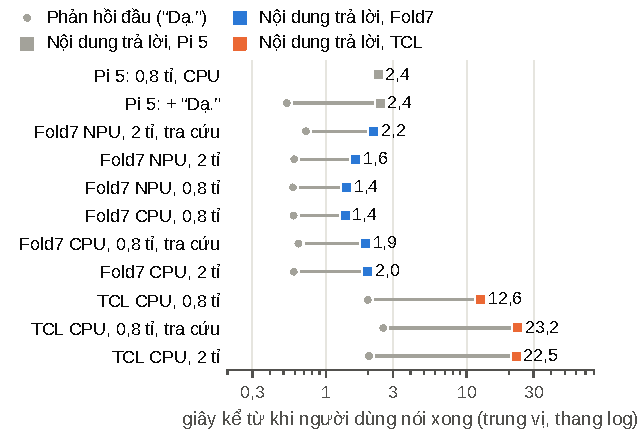
\includegraphics[width=\linewidth]{hai_may_latency.pdf}\par
{\scriptsize Trung vị, thang log. ``Dạ.'' được phát trước nội dung trả lời trên mọi thiết bị.}
\end{column}
\end{columns}
\end{frame}

% ------------------------------------------------------------------ 7
\begin{frame}{Thời gian đi đâu và so sánh bộ xử lý}
\begin{columns}[T]
\begin{column}{.48\textwidth}
\centering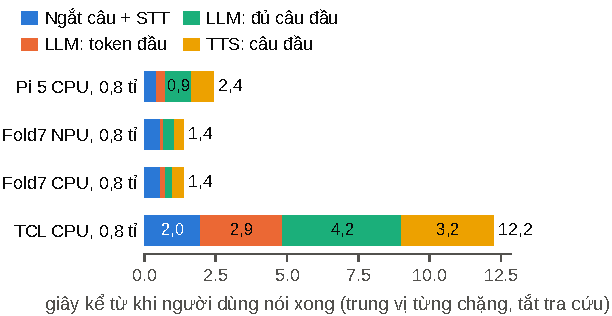
\includegraphics[width=\linewidth]{stages_v2.pdf}\par
{\scriptsize Cùng mô hình 0,8 tỉ, tắt tra cứu. Máy mạnh: chờ ngắt câu và STT chiếm nhiều nhất; TCL: mọi khâu đều chậm, LLM nặng nhất.}
\end{column}
\begin{column}{.48\textwidth}
\centering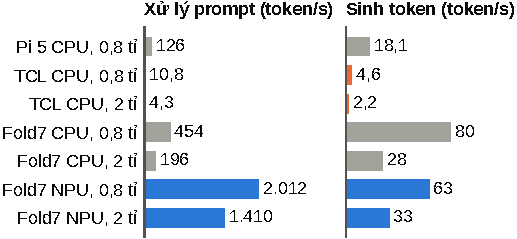
\includegraphics[width=\linewidth]{platform_v2.pdf}\par
{\scriptsize CPU 4 luồng trừ NPU. NPU xử lý prompt nhanh nên tra cứu gần như không làm tăng độ trễ; Cortex-A53 của TCL xử lý prompt chậm hơn Fold7 khoảng 42 lần.}
\end{column}
\end{columns}
\end{frame}

% ------------------------------------------------------------------ 8
\begin{frame}{Pi OS và Yocto-RT trên cùng Pi 5}
\begin{columns}[T]
\begin{column}{.47\textwidth}\footnotesize
\begin{tabular}{@{}lrr@{}}\toprule
Chỉ số & Pi OS & Yocto-RT\\\midrule
Đỉnh jitter, tải 30 ph (µs) & 127 & \textbf{92}\\
Trả lời, yên, p50 (s) & 1,60 & 2,02\\
RAM sau khởi động (MB) & 442-538 & \textbf{285}\\
Công suất, yên (W) & 3,03 & \textbf{2,78}\\
Xrun trên giờ & 0 & 0\\\bottomrule
\end{tabular}\par\vspace{6pt}
So cặp 16 câu: chênh 0,06\,s, Wilcoxon $p=0{,}40$. Yocto-RT cho sự cô lập lõi âm thanh, không cho tốc độ suy luận.
\end{column}
\begin{column}{.49\textwidth}
\centering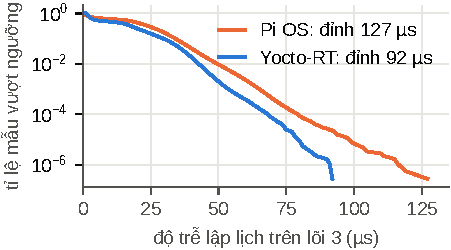
\includegraphics[width=\linewidth]{jitter.pdf}
\end{column}
\end{columns}
\end{frame}

% ------------------------------------------------------------------ 9
\begin{frame}{Kịch bản khẩn cấp khi mất kết nối}
\begin{columns}[T]
\begin{column}{.55\textwidth}
\begin{itemize}
\small
\item Mô hình nhỏ có tỉ lệ ảo giác 12\% đến 52\%: không chấp nhận được với ``con tôi bị rắn cắn''.
\item 85 thẻ: sơ cứu (rắn cắn, đuối nước, hồi sức tim phổi cho người lớn, trẻ em, sơ sinh…), thiên tai (bão, lũ quét, động đất, sóng thần), an toàn (gas, ngạt khí hầm, xả súng, phóng xạ, số khẩn cấp ở nước ngoài).
\item 82 nguồn: Bộ Y tế, Cục PCTT, Bộ Công an, Bạch Mai, MedlinePlus, CDC, NWS, WHO, Chữ Thập Đỏ…
\item Khớp: luật cụm từ có dấu, tổ hợp từ, bộ phân loại 10.832 câu; ASR thiên vị 1.276 cụm từ khẩn cấp.
\end{itemize}
\end{column}
\begin{column}{.42\textwidth}\small
\begin{tabular}{@{}lrr@{}}\toprule
Tập độc lập (khoá trước) & Văn bản & Giọng\\\midrule
v3, thẻ đợt 1 (114 câu) & 111 & 102\\
v4, 16 thẻ đợt 2 (64) & 64 & 47\\
v5, 9 thẻ quốc tế (36) & 35 & 30\\\bottomrule
\end{tabular}\par\vspace{4pt}
{\scriptsize Giọng: giọng tổng hợp rõ (WER 0,15 đến 0,22). Câu thường bị kích hoạt nhầm: 0/20 ở v4 và v5.}
\end{column}
\end{columns}
\end{frame}

% ------------------------------------------------------------------ 10
\begin{frame}{Thẻ an toàn trên hai điện thoại}
\centering\small
\begin{tabular}{@{}lcc@{}}\toprule
 & Galaxy Z Fold7 & TCL T506T\\\midrule
Kotlin giống Python (2.474 câu) & 2.474/2.474 & \tclParity\\
Thời gian khớp mỗi câu & 2,1\,ms & \tclParityMs\\
24 câu nói, thẻ mới: đúng thẻ & 20/24 & \tclSafeOk\\
24 câu nói, thẻ đợt 1: đúng thẻ & 20/24 & \tclSafeOkB\\
Phản hồi đầu p50 / chậm nhất & \hmSafeF{} / 0,61\,s & \tclSafeMed{} / \tclSafeMax\,s\\
Trong đó chờ ngắt câu + STT, p50 & 0,46\,s & \tclSttMed\,s\\\bottomrule
\end{tabular}\par\vspace{8pt}
\begin{minipage}{.9\textwidth}\small
Cùng câu sai trên cả hai máy (do nghe nhầm ``pin'' thành ``tinh'', ``suyễn'' thành ``diễn''), nên độ chính xác không phụ thuộc máy. Máy yếu chậm hơn ở khâu nhận dạng giọng nói: \tclSttNote
\end{minipage}
\end{frame}

% ------------------------------------------------------------------ 11
\begin{frame}{Điện thoại phổ thông TCL T506T: hỏi đáp tự do}
\centering\small
\begin{tabular}{@{}lccc@{}}\toprule
 & Fold7, 2 tỉ, NPU & TCL, 0,8 tỉ, CPU & TCL, 2 tỉ, CPU\\\midrule
Nạp mô hình & 6 đến 8\,s & \tclLoadA\,s & \tclLoadB\,s\\
Tốc độ sinh & 26 token/s & \tclTokA{} token/s & \tclTokB{} token/s\\
Nội dung trả lời, p50 & 1,53\,s & \tclAnsA\,s & \tclAnsB\,s\\
Bật tra cứu, nội dung trả lời & 1,53\,s & \tclAnsRag\,s & ---\\
Bộ nhớ ứng dụng lúc cao nhất & --- & \tclPssA\,GB & \tclPssB\,GB\\
Nhiệt độ pin sau bài thử & --- & \tclTempA\,°C & \tclTempB\,°C\\\bottomrule
\end{tabular}\par\vspace{8pt}
\begin{minipage}{.9\textwidth}\small\tclTakeaway\end{minipage}
\end{frame}

% ------------------------------------------------------------------ 11b
\begin{frame}{Máy mạnh và máy yếu: từng khâu, cùng đầu vào}
\begin{columns}[T]
\begin{column}{.56\textwidth}
\centering\small\setlength{\tabcolsep}{4pt}
\begin{tabular}{@{}lrr@{}}\toprule
Khâu & Fold7 & TCL T506T\\\midrule
STT, một câu (ms) & \hmAsrF & \hmAsrT\\
STT, hệ số thời gian thực & \hmAsrRtfF & \hmAsrRtfT\\
TTS, một câu (ms) & \hmTtsF & \hmTtsT\\
TTS, hệ số thời gian thực & \hmTtsRtfF & \hmTtsRtfT\\
Khớp thẻ, một câu (ms) & \hmSafeMsF & \hmSafeMsT\\
LLM 0,8 tỉ: nạp / sinh (token/s) & \hmPpF{} / \hmTgF & \hmPpT{} / \hmTgT\\
LLM 2 tỉ: nạp / sinh (token/s) & \hmPpBF{} / \hmTgBF & \hmPpBT{} / \hmTgBT\\
Nạp mô hình 0,8 tỉ (s) & \hmLoadF & \hmLoadT\\
Hỏi đáp: phản hồi đầu / nội dung (s) & \hmFirstF{} / \hmAnsF & \hmFirstT{} / \hmAnsT\\
Thẻ: đúng / phản hồi đầu (s) & \hmSafeOkF{} / \hmSafeF & \hmSafeOkT{} / \hmSafeT\\\bottomrule
\end{tabular}
\end{column}
\begin{column}{.40\textwidth}
\small
\begin{itemize}
\item Cùng tệp mô hình, cùng 24 câu khẩn cấp, 8 câu hỏi, cùng bộ đo; LLM đo bằng \texttt{llama-bench}, CPU 4 luồng.
\item Độ chính xác không đổi: 2.474/2.474 câu khớp thẻ giống nhau trên hai máy.
\item Câu khẩn cấp không qua LLM nên máy yếu vẫn có tiếng sau \hmSafeT\,s.
\item Hỏi đáp tự do chậm \hmSpeedup{} lần: bản cho máy chỉ có CPU tắt tra cứu và lịch sử.
\end{itemize}
\end{column}
\end{columns}
\end{frame}

% ------------------------------------------------------------------ 11c
\begin{frame}{Sản phẩm chạy trên điện thoại thật}
\centering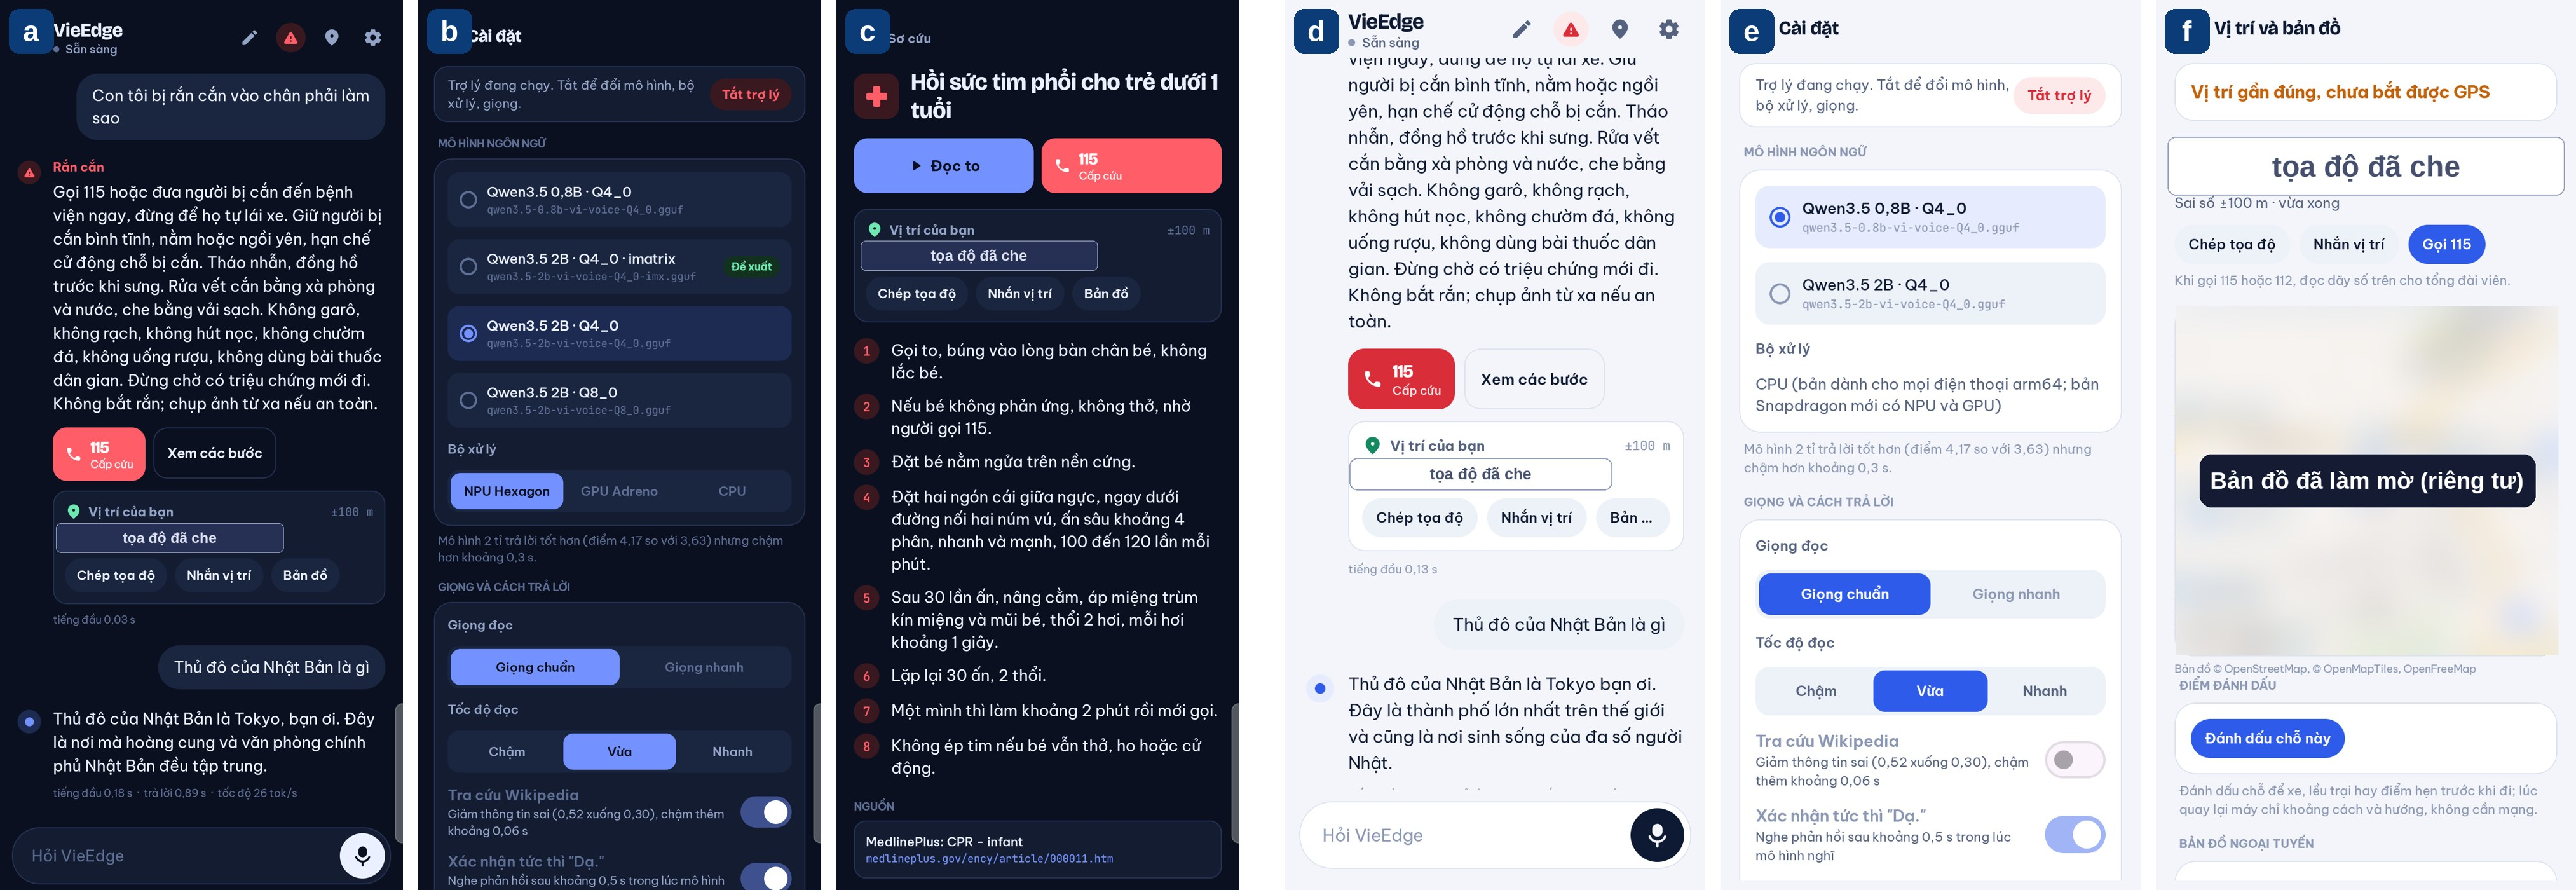
\includegraphics[width=\textwidth]{anh_may.jpg}\par\vspace{6pt}
\begin{minipage}{.95\textwidth}\footnotesize
Ảnh chụp màn hình trực tiếp từ máy. Galaxy Z Fold7: (a) câu khẩn cấp trả lời bằng thẻ có nút gọi 115 và vị trí, rồi câu hỏi tự do qua LLM; (b) cài đặt, mô hình 2 tỉ trên NPU Hexagon; (c) thẻ hồi sức tim phổi cho trẻ dưới 1 tuổi kèm nguồn. TCL T506T: (d) cùng hai câu hỏi; (e) bản dựng chỉ dùng CPU; (f) vị trí và bản đồ ngoại tuyến. Tọa độ được che, bản đồ làm mờ vì là vị trí thật.
\end{minipage}
\end{frame}

% ------------------------------------------------------------------ 12
\begin{frame}{Tính năng mới: vị trí GPS và bản đồ ngoại tuyến}
\begin{columns}[T]
\begin{column}{.55\textwidth}
\small
\begin{itemize}
\item GPS không cần sóng điện thoại hay Wi-Fi: máy báo có tín hiệu không, bao nhiêu vệ tinh, sai số bao nhiêu mét.
\item Tọa độ hiện trên mọi câu trả lời khẩn cấp để đọc cho 115, có nút chép và nhắn tin vị trí; hỏi ``tôi đang ở đâu'' thì trợ lý đọc tọa độ.
\item Mất tín hiệu (hang, thung lũng, trong nhà): giữ vị trí gần nhất kèm thời gian.
\item Bản đồ ngoại tuyến: tải trước vùng 10 đến 50 km khi còn mạng (OpenFreeMap, giới hạn 3.000 mảnh, 50 MB mỗi lần); đánh dấu chỗ để xe, lều trại và chỉ khoảng cách, hướng quay lại.
\end{itemize}
\end{column}
\begin{column}{.40\textwidth}
\footnotesize
\begin{block}{Vì sao không dùng máy chủ OpenStreetMap?}
Chính sách của máy chủ tile.openstreetmap.org cấm tải trước để dùng ngoại tuyến; OpenFreeMap cho phép trong giới hạn trên.
\end{block}
\vspace{6pt}
\begin{block}{Đo trên TCL T506T}
Vùng 25 $\times$ 25\,km: 224 mảnh, 30,8\,MB, khoảng 45\,s qua Wi-Fi. Tắt Wi-Fi: bản đồ vẫn hiện cả khu vực chưa từng xem. Trong nhà không bắt được GPS, máy dùng vị trí gần đúng từ mạng (sai số khoảng 100\,m) và báo rõ điều đó.
\end{block}
\end{column}
\end{columns}
\end{frame}

% ------------------------------------------------------------------ 13
\begin{frame}{Những gì đã thử mà không hiệu quả}
\begin{itemize}
\item Encoder PhoWhisper trên Hailo-8L: cosine 0,84 so với ONNX, dưới ngưỡng 0,9.
\item Giải mã suy đoán: 13,9 so với 14,3 token/s, không nhanh hơn.
\item LLM chọn thẻ an toàn: đúng 2/126 câu, kích hoạt nhầm 140/345.
\item Lời nhắc yêu cầu trả lời trực tiếp: câu mở đầu ``Mình không chắc'' giảm từ 252 xuống 21 trên 345, nhưng tỉ lệ ảo giác tăng từ 21\% lên 48\% (giám khảo 9 tỉ). Giữ lời nhắc ưu tiên tính trung thực.
\item Gemma-4-E2B: ảo giác ít hơn (5\% câu văn bản) nhưng trên Fold7 cần 6 đến 7,5\,s mới có câu trả lời.
\end{itemize}
\end{frame}

% ------------------------------------------------------------------ 14
\begin{frame}{Kết luận}
\begin{itemize}
\item Hỏi đáp tiếng Việt chạy ngoại tuyến đầu cuối trên Pi 5, Fold7 và cả điện thoại phổ thông 4\,GB RAM.
\item Câu khẩn cấp: thẻ có nguồn, đúng thẻ 97\% đến 100\% với văn bản; phản hồi đầu \hmSafeF\,s trên Fold7, \hmSafeT\,s trên TCL.
\item Máy mạnh và máy yếu cùng độ chính xác; máy yếu chậm \hmSpeedup{} lần ở hỏi đáp tự do.
\item Khâu yếu nhất là nghe: giọng tổng hợp kém chỉ 48\%, giọng rõ 89,5\%; giọng người thật chưa đo.
\item Hạn chế: thẻ chưa được nhân viên y tế duyệt; câu thử do nhóm viết; 24 câu nói mỗi máy.
\item Tiếp theo: thu giọng người thật trên điện thoại, nhờ bác sĩ duyệt thẻ, thử trên nhiều máy phổ thông hơn.
\end{itemize}
\vspace{10pt}
\begin{center}{\Large\bfseries\color{dam}Cảm ơn thầy cô và các bạn đã lắng nghe}\end{center}
\end{frame}

\end{document}
